\chapter{Problem 1}
  \section{Problem 1a}
	
	From the z-transform of the described filter in Problem 1 we get:
	\begin{equation}
		X(z)=\rho X(z)z^{-1}+\sqrt{1-\rho ^2}*E(z) 
		\label{eq:eq_impulse_response}
	\end{equation}
	If we sort equation~\ref{eq:eq_impulse_response} in regard of $\frac{X(z)}{E(z)}$ we get:
	\begin{equation*}
		\frac{X(z)}{E(z)}=\frac{\sqrt{1-\rho ^2}}{1-\rho z^{-1}}
		\label{eq:eq_freq_resp_x}
	\end{equation*}
	
	Make the z-transform back to the diskrete plane
	
	\begin{equation*}
		h(n)=\sqrt{1-\rho ^2}\rho ^nu(n)
	\end{equation*}
	
	Since the noise is uncorrolated, we may reduce the convolution to find x(n)
	
	\begin{equation*}
		x(n)=h(n)\Asterisk e(n)=h(n)\sigma ^2_W
	\end{equation*}
	
	From Problem 1 it is given that
	
	\begin{equation*}
		\sigma ^2_W=1
	\end{equation*}
	
	This results in the following expression for x(n):
	
	\begin{equation}
		x(n)=\sqrt{1-\rho ^2}\rho ^nu(n)
		\label{eq:eq_AR_process}
	\end{equation}
	
	From the output calculated in equation~\ref{eq:eq_AR_process} we may use the following formula from the compendium to calculate the autocorrelation:
	
	\begin{equation}
		R_x(\tau)=\sum_{n=-\infty}^{\infty}E\{x(n)\}E\{x(n+\tau)\}
		\label{eq:eq_autocorrelation_compendium}
	\end{equation}
	
	By inserting our definition of x(n) we get the following equation:
	
	\begin{equation*}
		R_x(\tau)=(1-\rho ^2)\sum_{n=0}^{\infty}\rho ^n\rho^{n+\tau}
	\end{equation*}
	
	By using the formula for geometric series we conclude with this resulting formula:
	
	\begin{equation*}
		R_x(\tau)=(1-\rho ^2)\rho^{\tau }\sum_{n=0}^{\infty}\rho^{2n}=(1-\rho ^2)\rho^{\tau }\frac{1}{1-\rho ^2}
	\end{equation*}
	
	After shorting down the last equation, this is the complete answer:
	
	\begin{equation}
		R_x(\tau)=\rho^{|\tau |}
	\end{equation}
	
	\lstinputlisting{Matlab/oppgave1a.m}
	
	\begin{figure}[H]
	  \centering
	  \includegraphics[width=0.75\textwidth]{img/Oppgave1a}
	\end{figure}
	
  
  
  \section{Problem 1b}
	From the compendium we have that the power spectral density may be given by the following formula:
	\begin{equation}
		Sx(f)=|H(f)|^2=H(f)H^*(f)
	\end{equation}
	
	Insert the expression from equation~\ref{eq:eq_freq_resp_x} and calculate:
	
	\begin{equation*}
		H(f)=H(z)|_{z=e^{j2\pi f}}=\frac{\sqrt{1-\rho ^2}}{1-\rho e^{-j2\pi f}}
	\end{equation*}
	
	Expanding the denominator and cleaning up.
	
	\begin{equation*}
		Sx(f)=\frac{\sqrt{1-\rho ^2}^2}{(1-\rho e^{-j2\pi f})(1-\rho e^{j2\pi f})}=\frac{1-\rho ^2}{1-\rho e^{j2\pi f}-\rho e^{-j2\pi f}+\rho ^2}
	\end{equation*}
	
	Using eulers formula for cosine function to reduce the equation to the following result:
	
	\begin{equation}
		Sx(f)=\frac{1-\rho ^2}{1+\rho ^2-2\rho cos(2\pi f)}
		\label{eq:eq_Spectral_Density_X}
	\end{equation}
	
	\lstinputlisting{Matlab/Oppgave1b.m}
	
	\begin{figure}[H]
	  \centering
	  \includegraphics[width=0.75\textwidth]{img/Oppgave1b}
	\end{figure}
  
  \section{Problem 1c}
  
	\lstinputlisting{Matlab/Oppgave1c.m}
  
  \section{Problem 1d}
  
	\lstinputlisting{Matlab/Oppgave1d.m}
	
	\begin{figure}[h]
	  \centering
	  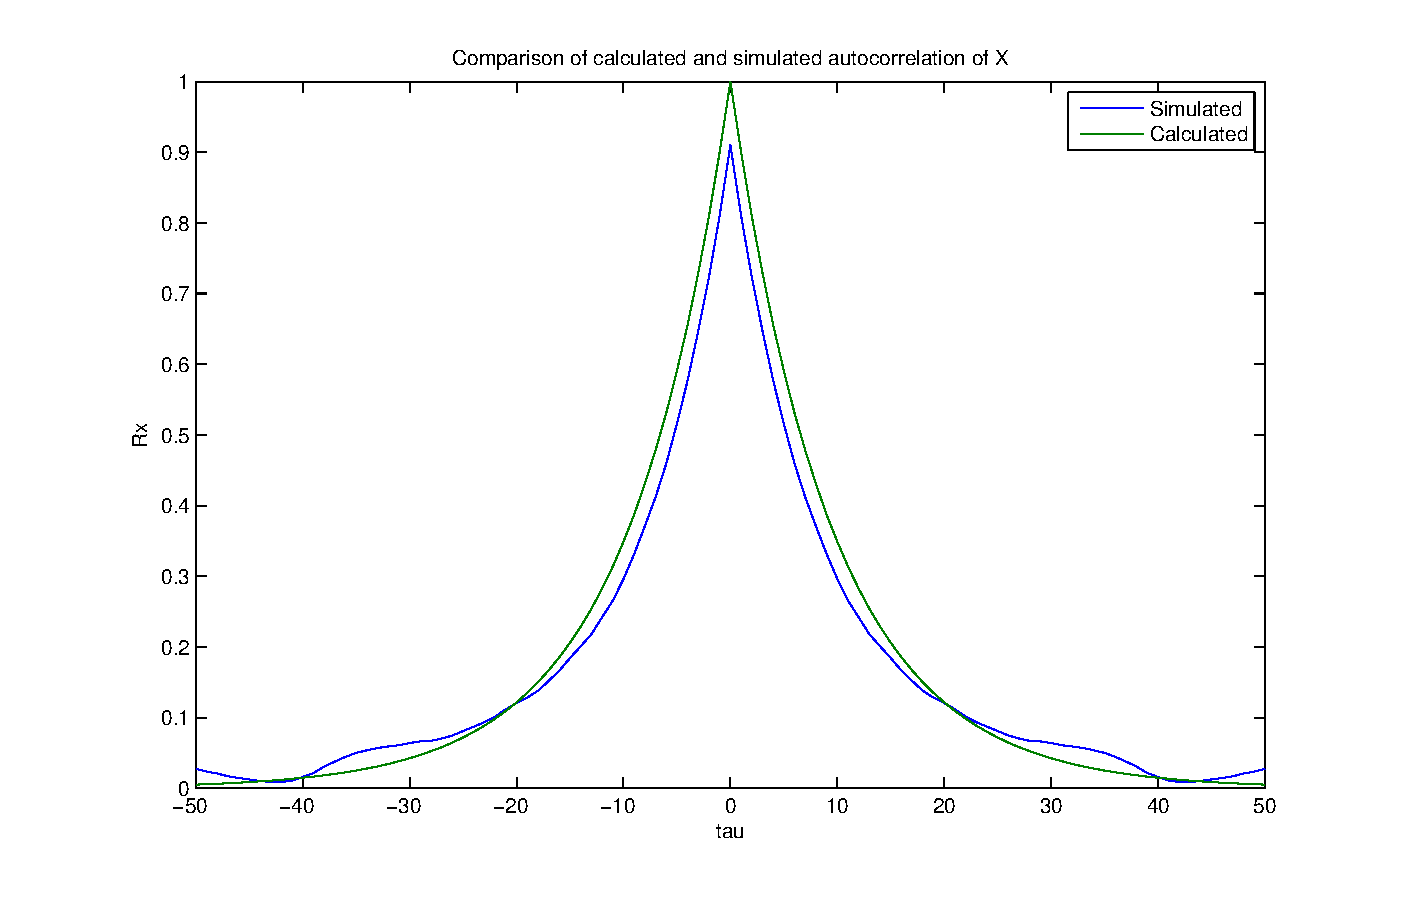
\includegraphics[width=0.75\textwidth]{img/Oppgave1d}
	\end{figure}
  
  \section{Problem 1e}
  
	\lstinputlisting{Matlab/Oppgave1e.m}
	
	\begin{figure}[h]
	  \centering
	  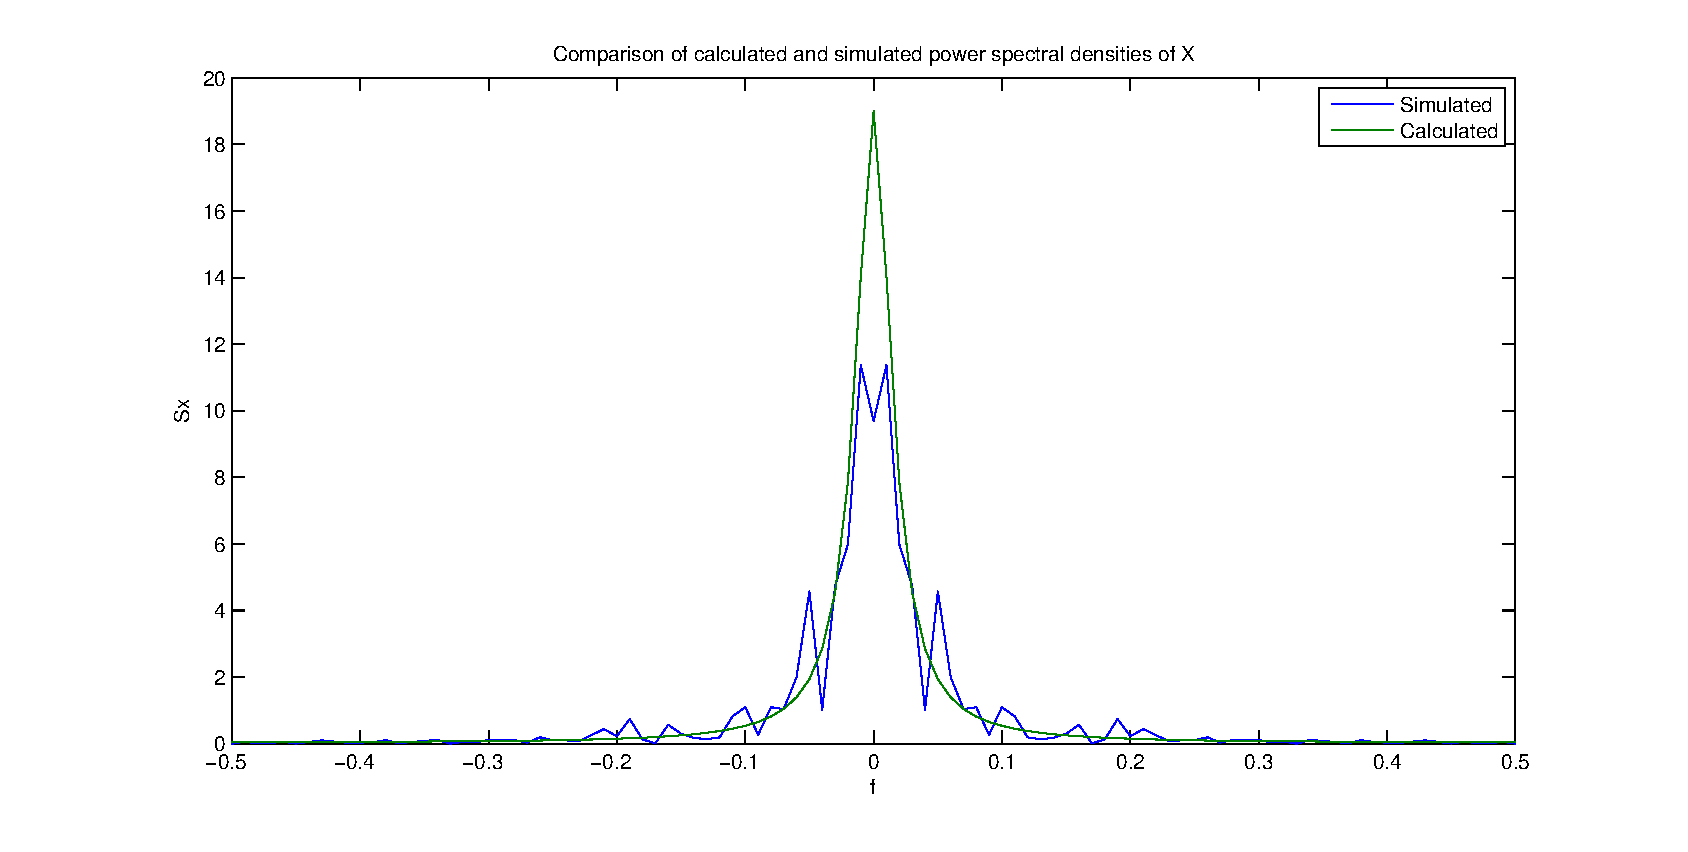
\includegraphics[width=0.75\textwidth]{img/Oppgave1e}
	\end{figure}